\documentclass{ximera}

\author{Bart Snapp}

\title{M\"obius strip}

\begin{document}
\begin{abstract}
  As a group you will make a M\"obius strip.
\end{abstract}
\maketitle

As a group, you will put your heads together to produce a plot like this one:
\begin{image}
  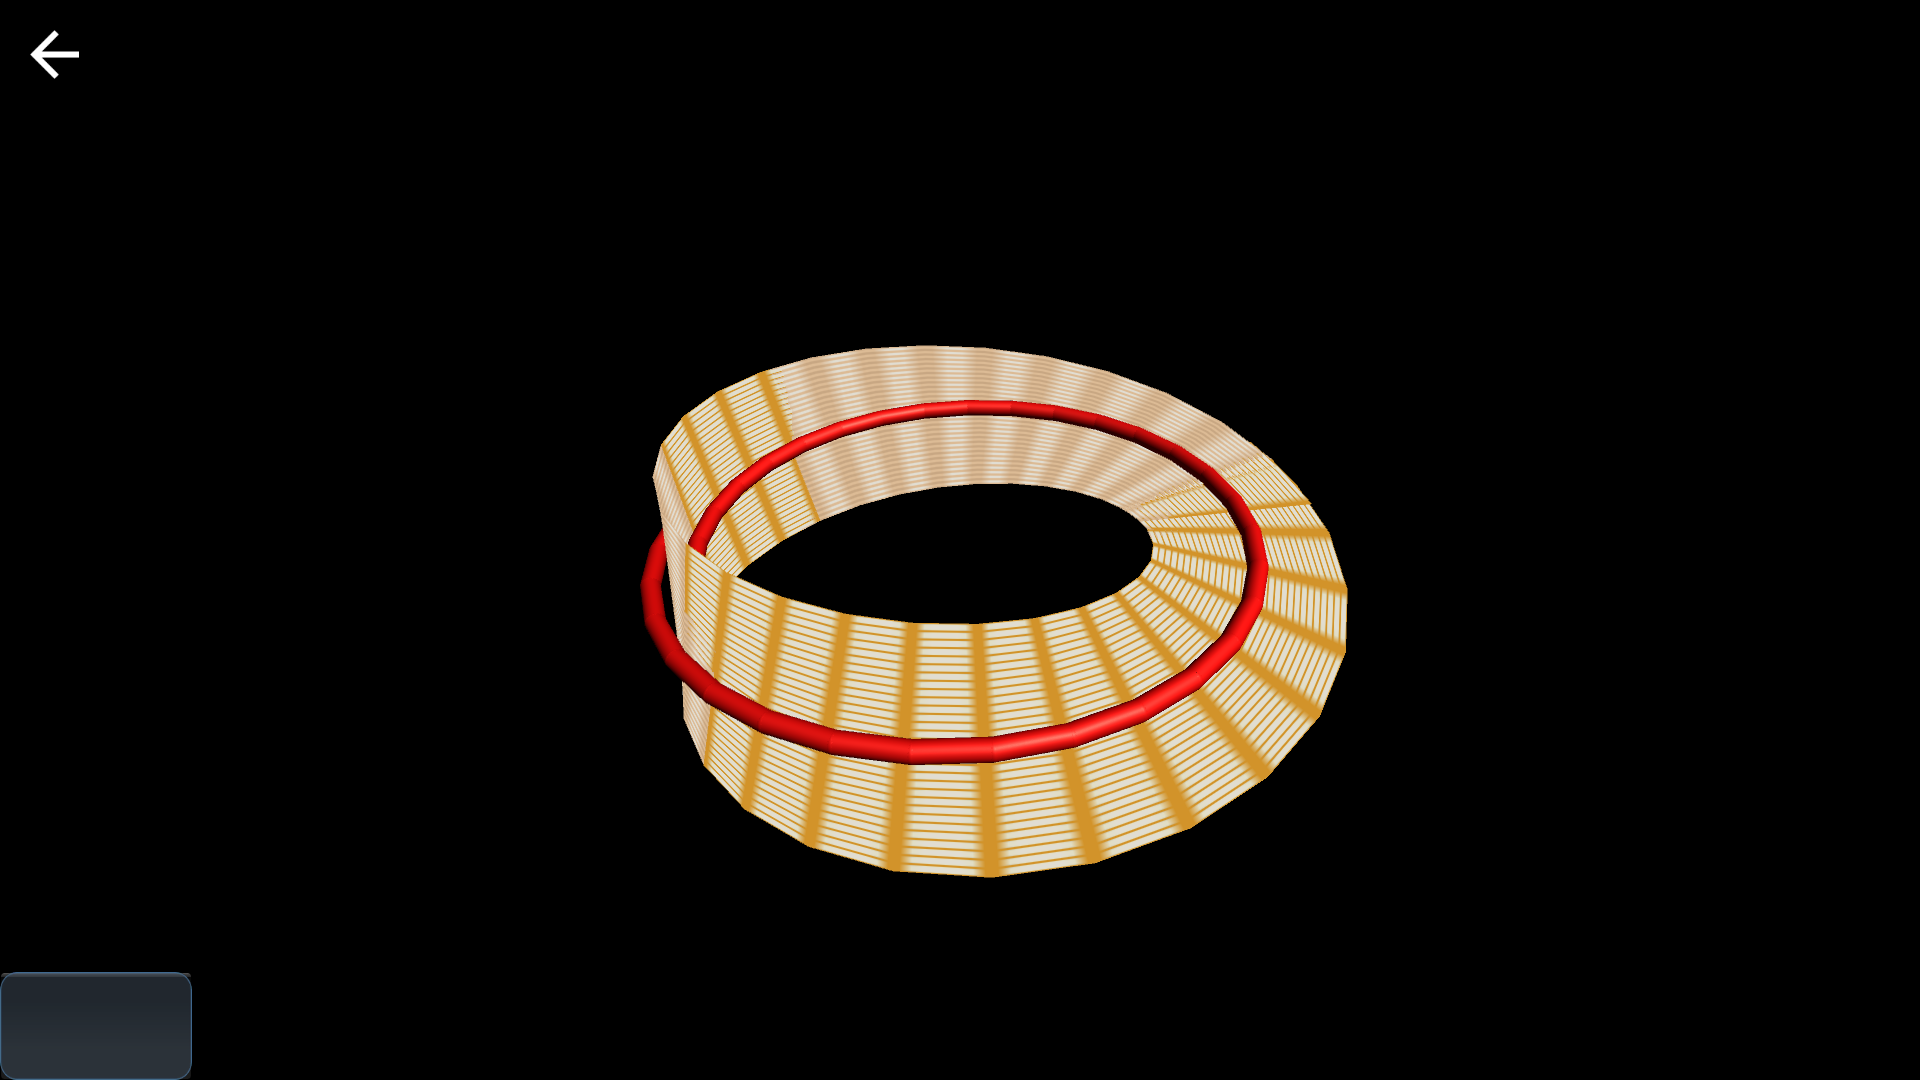
\includegraphics{mobius.png}
\end{image}

Use this parametric formula for the M\"obius strip:
\begin{align*}
  x(s,t) &= (3+s\cdot \cos(t/2))\cos(t)\\
  y(s,t) &=(3+s\cdot \cos(t/2))\sin(t)\\
  z(s,t) &=s\cdot \sin(t/2),
\end{align*}
where $0\le t<2\pi$ and $-1\le s\le 1$. You can learn more about the
M\"obius strip \link[here]{http://mathworld.wolfram.com/MoebiusStrip.html} and \link[here]{https://en.wikipedia.org/wiki/Mobius_strip}.

Your task is to put a curve, floating above the center of the strip,
$1/5$ of a unit away. This curve will actually travel \textit{twice}
the length of the unfolded M\"obius strip, since the strip itself is
\textit{one-sided}!
\end{document}
